\newpage
\section*{Ziel}
Es soll die Federrate einer Zugfeder im Hinblick auf die Paramter der Federdicke und der Windungszahl
untersucht werden. Somit soll rückschließend ein Möglichkeit zur Materialeinsparung 
innerhalb eines vorgegebenen Ratentoleranzbereich gefunden werden.  

\section{Zugfedern allgemein}
Überall wo die Krafteinwirkung nicht auf Druck, sondern auf Zug erbracht werden muss
werden Zugfedern verwendet. Trotz der benötigten Größe des Einbauraumes und der sensiblen
Stelle an den Ösen, werden Zugfedern vor allem aufgrund ihrer Knickfreiheit verwendet.
Führungselemente wie Hülsen oder Dorn sind somit überflüssig und somit besteht die Möglichkeit
einer reibungsfreien zentrischen Kraftübertragung.\\
IM folgenden soll kurz auf die verschiedenen Komponenten und Unterschiede zwischen
ZUgfedern eingegangen werden:
\begin{enumerate}
    \item Federbauform und Ösenform
    \item Vorspannung
    \item Relaxation, Schubspannung und Federkräften
    \item Belastungsart
    \item Federwerkstoff und Oberfläche
\end{enumerate}



\subsection{Federbauform}
Die gängigen Federbauformen für Zugfedern sind zylindrischer Form mit einer linearen
Federkennline, aber auch kegel- oder tonnenförmige Formen sind verbreitet, was vorallem
den Vorteil einer höhren Lebensdauer hat.
\begin{figure}[H]
    \centering
    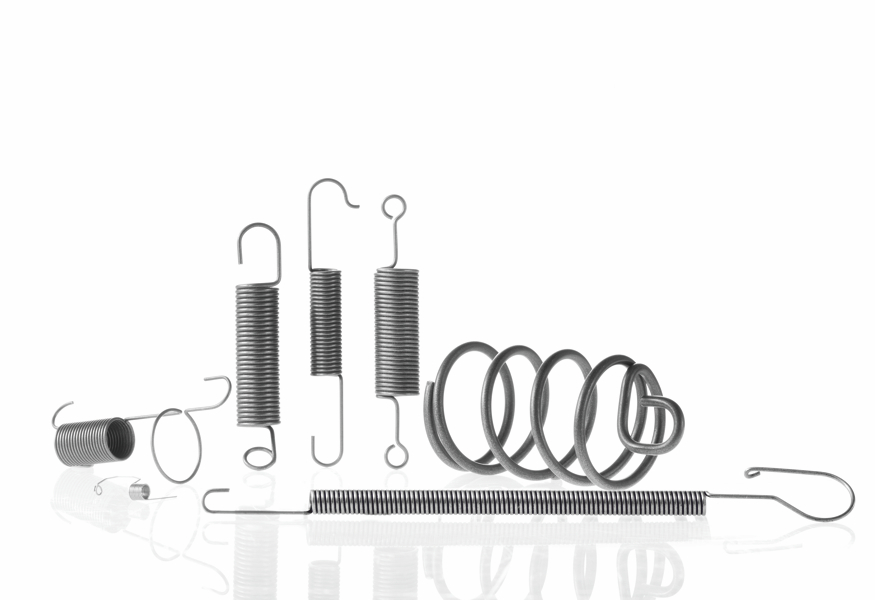
\includegraphics[width=0.6\textwidth]{bilder/Input/zugfedern_spezial.jpg}
    \caption{Spezielle Zugfedern \cite{KompZ}}
\end{figure}



\subsection{Ösenform}
Die Ösen der Zugfedern (bzw. die Ösenanbindung am Übergangsbogen) bilden eine schwierige Region, da es dort oftmal zu Ösenbrüchen
kommen kann. Aufgrund dessen sind Zugfedern nicht für Dauerfest-Einsätze geeignet.
Als klassisch gilt die 1/1 deutsche Öse oder der Hakenöse.
Für eine erhöhte Lebensdauer verwendet man auch einen eingerollten Gewindebolzen 
oder einen eingeschraubte Gewindestopfen.\\
Die Öse bildet dabei den zentralen Angriffspunkt für drei Kräfte: Zugbelastung, Torsionsbelastung und Biegebelastung.
\begin{figure}[H]
    \centering
    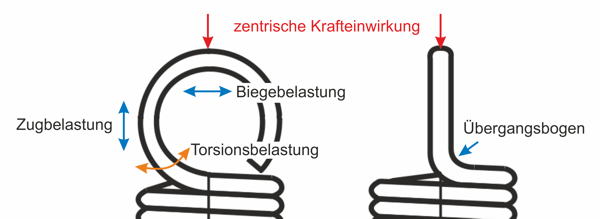
\includegraphics[width=0.6\textwidth]{bilder/Input/Oesenbelastung.jpg}
    \caption{Verschiedene Ösenbelastungen \cite{KompZ}}
\end{figure}
\begin{figure}[H]
    \centering
    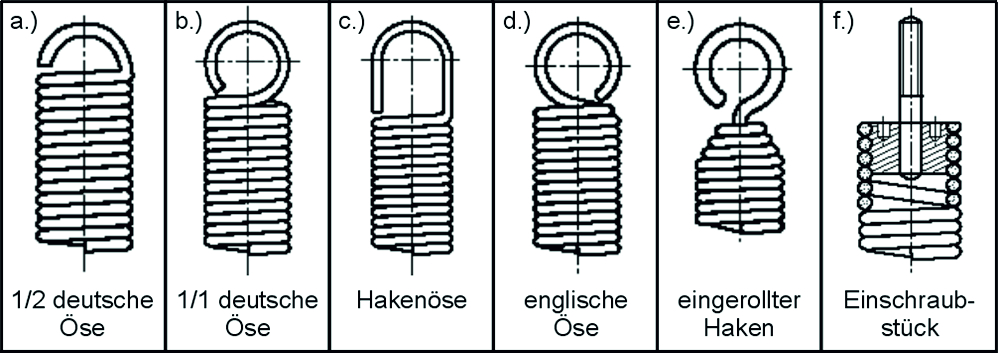
\includegraphics[width=0.6\textwidth]{bilder/Input/Oesenformen.jpg}
    \caption{Verschiedene Ösenformen \cite{AusM2}}
\end{figure}


\subsection{Beanspruchungsart}
Generell unterscheidet man zwischen einer statischen und einer dynamischen Beanspruchung.
Von einer statischen Beanspruchung einer Zugfeder sricht man bei einer zeitlich
konstanten Belastung, bzw. einer Belastung mit weniger als 10000 Hüben oder 
kleinen Hubspannungen.
Hat die Feder mehr als 10000 Lastwechsel oder Hubspannungen die konstanten und veränderlichen sind,
so spricht man von einer dynamischen Beanspruchung.
\newpage


\subsection{Vorspannung}
Bei der Herstellung entsteht eine Vorspannung ufgrund eines Drilles gegen die nächste
Windung. Dadurch wird die Betribslänge der Zugfeder minimiert, sie ist allerdings mit höhren Produktionskosten
verbunden.
\begin{figure}[H]
    \centering
    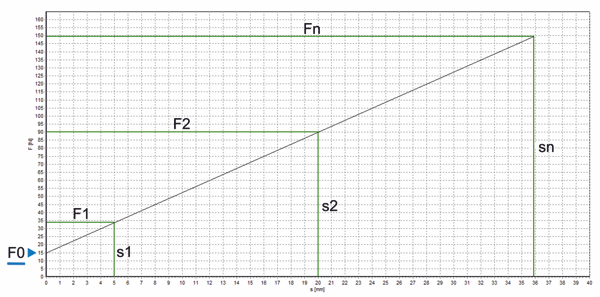
\includegraphics[width=0.6\textwidth]{bilder/Input/Vorspannung.jpg}
    \caption{Zugfeder Weg-Kraft-Diagramm \cite{KompZ}}
\end{figure}




















%THEORIE ----------------------------------------------------------------------
\newpage
\section{Theorie}
\begin{figure}[H]
    \centering
    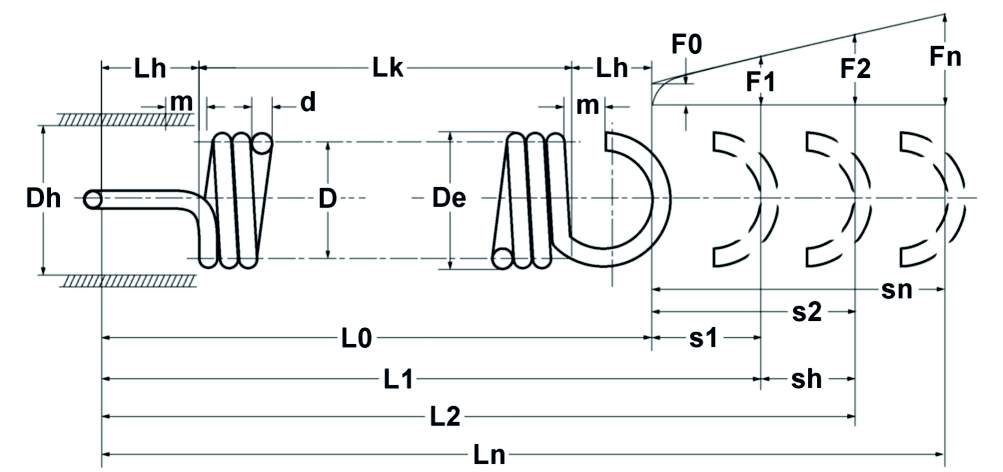
\includegraphics[width=0.6\textwidth]{bilder/Input/Zugfeder_technisch.jpg}
    \caption{Theoretisches Zugfederdiagramm \cite{AusM2}}
\end{figure}
Für zylinderische Zugfedern aus Draht mit einem Kreisquerschnitt gilt:\\\\

Die Federrate (auch Federkonstante) $R$:
\begin{equation}
    %Federrate
    R=\frac{F}{s}=\frac{Gd^4}{8D^3n}=\frac{F-F_0}{s}
    \label{eqn:federrate}
\end{equation}

Die Federkraft $F$:
\begin{equation}
    %Federkraft
    F=\frac{Gd^4s}{8D^3n}+F_0=R \cdot s +F_0
    \label{eqn:federkraft}
\end{equation}

Der Federweg $s$:
\begin{equation}
    %Federweg
    s=\frac{8D^3(F-F_0)}{GD^4}
    \label{eqn:federweg}
\end{equation}

Für den Festigkeitsnachweis der Zugfeder ist die Ermittlung der Schubspannung $\tau$
nötig, welche für die dynamischenBeanspruchungen mit einem Faktor $k$ korrigiert werden müssen.

\begin{equation}
    %Schubspannung
    \tau = \frac{8DF}{\pi d^3}
    \label{eqn:schubspannung}
\end{equation}
\begin{align}
    \tau_k &= k \cdot \tau\\
    \text{mit }k&=\frac{\frac{D}{d}+0.5}{\frac{D}{d}-0.75}
\end{align}
Für die zulässige Spannung ergib sich
\begin{equation}
    \tau_{zul}=0.45 \cdot R_m
\end{equation}
Dabei spiegelt $R_m$ die ZUgfestigkeit des Federstahls wieder.\\
Ist dabei $s_n$ der zu $\tau_{zul}$ Federweg, so sollte in der Praxis nur 80\% dieses
Federweges ausgnutzt werden um Relaxation (Kraftverlust) zu vermeiden.
Also $s_{prax}=0.8 \cdot s_n$  




\label{sec:theorie}